\documentclass[10pt,oneside]{book}
% \usepackage[a4paper, left=25mm,right=25mm,top=25mm,bottom=25mm]{geometry}
\usepackage[a4paper]{geometry}
% \usepackage[utf-8]{inputenc}
\usepackage{amsmath}
\usepackage{amssymb}
\usepackage{cite}
\usepackage{graphicx}
\usepackage{hyperref}
\usepackage{mdframed}
\usepackage{titlesec}
\usepackage{xcolor}

%%%%%%%%%%%%%%%%%%%%%%%%%%%%%%%%%%%%%%%%%%%%%%%%%%%%%%%%%%%%%%%%%%%%%%%% Setups
\newcommand{\Eq}[1]{Equation~\ref{eq:#1}}
\newcommand{\Fig}[1]{Figure~\ref{fig:#1}}

\newenvironment{book_quote}[1]
{%
  \mdfsetup{%
    frametitle={\colorbox{white}{\space#1\space}},
    frametitleaboveskip=-\ht\strutbox,
  }
  \begin{mdframed}
}
{
  \end{mdframed}
}

\graphicspath{{./fig/}}

\hypersetup{%
  bookmarksopen=true,
  linktoc=all,
  pdfauthor=Jihang Li,
}

\title{Notes of Concepts and Representations in Vision and Cognition}
\author{Jihang Li}
%%%%%%%%%%%%%%%%%%%%%%%%%%%%%%%%%%%%%%%%%%%%%%%%%%%%%%%%%%%%%%%%%%%%%%%%%%%%%%%

\begin{document}
\maketitle
\tableofcontents

%%%%%%%%%%%%%%%%%%%%%%%%%%%%%%%%%%%%%%%%%%%%%%%%%%%%%%%%%%%%%%%%%%%%%%%% Part 1
\part{Low and Mid Level Vision}%


%%%%%%%%%%%%%%%%%%%%%%%%%%%%%%%%%%%%%%%%%%%%%%%%%%%%%%%%%%%%%%%%%%%%%%%% Part 2
\part{Stochastic Grammars in Vision}%
%==================================================================== Chapter 1
\chapter{Overview of Stochastic Grammar}%
\label{sec:ii.1}
Statistical grammar is a framework with \textbf{probabilistic notion} of
grammaticality.

\section{The Origin of Grammars}%
\label{sec:ii.1.1}
Signals $s$ in real world that tend to occur together more frequently than by
chance can be grouped together to form higher order parts of the signal, and
this process can be repeated to form larger parts. This form a vocabulary of
\textbf{``reusable''} parts.

To measure whether a grouping is a good part:
%
\begin{align}
  \label{eq:ii.1.1}
  \log_2 \left( \frac{p(s\vert_{A \cup B})}{p(s\vert_{A}) \cdot p(s\vert_{B})} \right)
\end{align}
%
where $s\vert_{A}$ and $s\vert_{B}$ are two parts of signal $s: D \rightarrow I$,
with $A \subset D$ and $B \subset D$. Two parts of a signal are bound if the
probability of their co-occurrence is significantly \textbf{greater than} the
probability if their occurrence was independent. Example as shown in
\Fig{ii.1.1}.
%
\begin{figure}[!htpb]
  \centering
  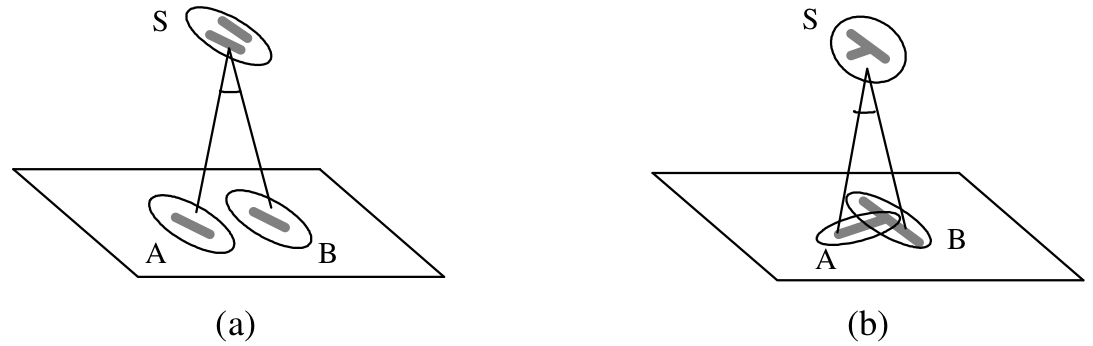
\includegraphics[width=0.8\linewidth]{./fig/fig_ii_1_1.png}
  \caption{(a) Two parallel lines form a reusable part containing as its
    constituents the two lines (b) A T-junction is another reusable part formed
    from two lines.}%
  \label{fig:ii.1.1}
\end{figure}
%

\begin{book_quote}{\textit{Original Texts}}
  The set of such reusable parts is called the \textbf{parse graph} of the
  signal. Firstly, associate to a signal $s$ the set of subsets $\{A_i\}$ of
  $D$ such that $s\vert_{A_i}$ is a reusable part. Then these subsets are made
  into the nodes $\langle A_i \rangle$ of the parse graph. In the graph, the
  proper inclusion of one subset in another, $A_i \subsetneqq A_j$, is shown by
  a ``vertical'' directed edge
  $\langle A_j \rangle \rightarrow \langle A_i \rangle$. For simplicity, we
  prune redundant edges in this graph by adding edges only when
  $A_i \subsetneqq A_j$ and there is no $A_k$ such that
  $A_i \subsetneqq A_k \subsetneqq A_j$.

  \par
  In the ideal situation, parse graph is a tree with the whole signal at the
  top and the domain D (the letters of the text or the pixels of the image) at
  the bottom. Moreover, each node $\langle A_i \rangle$ should be the disjoint
  union of its children, i.e., the parts $\{A_j \vert A_j \subsetneqq A_i\}$
  such that $\cup_j A_j = A_i$.
\end{book_quote}

\section{The Traditional Formulation of Grammar}%
\label{sec:ii.1.2}
Grammar $\mathcal{G} = (V_N, V_T, \mathbf{R}, S)$, where $V_N$ is a finite
set of non-terminal nodes, $V_T$ is a finite set of terminal nodes, $S \in V_N$
is a start symbol at the root, and \textbf{R} is a set of production rules,
%
\begin{align}
  \label{eq:ii.1.2}
  \mathbf{R} = \{\gamma: \alpha \rightarrow \beta\}
\end{align}
%
where $\alpha, \beta$ are strings that
$\alpha, \beta \in {(V_N \cup V_T)}^+$\footnote{$V^*$ means a string consisting
of $n \geq 0$ symbols from $V$, and $V^+$ means $n \geq 1$} and including at
least one non-terminal symbol. Chomsky classified languages into 4 types
according to the form of their production rules:
%
\begin{itemize}
  \item Definition: $A, B \in V_N$, $a \in V_T$
  \item Type 0: a \textbf{phrase structure or free} grammar with no constraint
    on $\alpha$ and $\beta$
  \item Type 1: a \textbf{context sensitive} grammar, where
    $\xi A \eta \rightarrow \xi \beta \eta$ means $A$ is rewritten by $\beta$
    in the context of strings $\xi$ and $\eta$
  \item Type 2: a \textbf{context free} grammar, $A \rightarrow \beta$
  \item Type 3: a \textbf{finite state or regular} grammar,
    $A \rightarrow aB$ or $A \rightarrow a$
\end{itemize}
%

The set of all possible strings of terminals $\omega$ derived from a
$\mathcal{G}$ is called its \textbf{language}:
%
\begin{align}
  \label{eq:ii.1.3}
  \mathbf{L}(\mathcal{G}) = \{\omega: S \overset{\mathbf{R^*}}{\implies} \omega, \omega \in V^*_T\}
\end{align}
%
$\mathbf{R^*}$ means a sequence of production rules deriving $\omega$ from $S$:
%
\begin{align}
  \label{eq:ii.1.4}
  S \overset{\gamma_1, \gamma_2, \ldots, \gamma_{n(\omega)}}{\implies} \omega
\end{align}
%
If $\mathcal{G}$ is of type 1, 2 or 3, then a \textbf{parse tree} is obtained
for a given $\omega$:
%
\begin{align}
  \label{eq:ii.1.5}
  \mathbf{p}t(\omega) = (\gamma_1, \gamma_2, \ldots, \gamma_{n(\omega)})
\end{align}
%

For example, in images, $V_T$ can be pixels or a simple set of local structures
in the images such as textons and other image primitives. Then $V_N$ will be
reusable parts and objects in the image. And a production rule
$A \rightarrow \beta$ is a template which enables you to expand A. Then
$\mathbf{L}(\mathcal{G})$ will be the set of all valid object
\textbf{configurations}.

The grammar rules represent both structural \textbf{regularity} and
\textbf{flexibility}:
%
\begin{itemize}
  \item Regularity: enforced by the template which decomposes an entity $A$,
    such as object into certain elements in $\beta$
  \item Flexibility: reflected by the fact that each structure $A$ has many
    alternative decompositions
\end{itemize}
%

A parse tree:
%
\begin{itemize}
  \item Root is an Or-node
  \item Or-nodes are labelled by $V_N \cup V_T$
  \item And-nodes are labelled by $\mathbf{R}$
\end{itemize}
%
To generate a parse tree:
%
\begin{enumerate}
  \item For any Or-node with $A$, consider all rules have $A$ on the left and
    create children which have And-nodes labelled by corresponding rules.
  \item Step 1 expand to a set of Or-nodes labelled by the symbols on the right
    of the rule.
  \item An Or-node labelled by terminal does not expand further.
\end{enumerate}
%
\begin{figure}[!htpb]
  \centering
  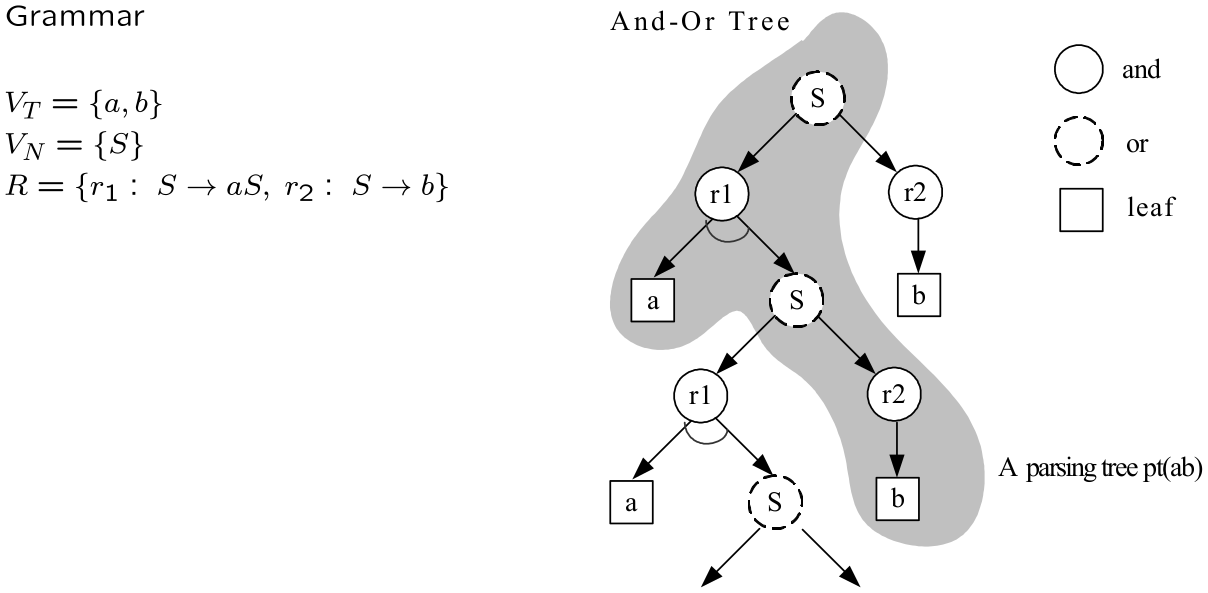
\includegraphics[width=0.7\linewidth]{./fig/fig_ii_1_2.png}
  \caption{A very simple grammar, its universal And-Or tree and a specific
    parse tree in shadow.}%
  \label{fig:ii.1.2}
\end{figure}
%

A vision example of an And-Or tree, using the reusable parts in
\Fig{ii.1.1}, us shown in \Fig{ii.1.3}. $B, C$ are the two ambiguous ways to
interpret $A$. $B$ represents an occlusion configuration with two layers while
$C$ represents a butting/alignment configuration at one layer.  $A$ is a
\textbf{frequently observed local structure} in natural images when a long bar
(e.g.\ a tree trunk) occludes a surface boundary (e.g.\ a fence).
%
\begin{figure}[!htpb]
  \centering
  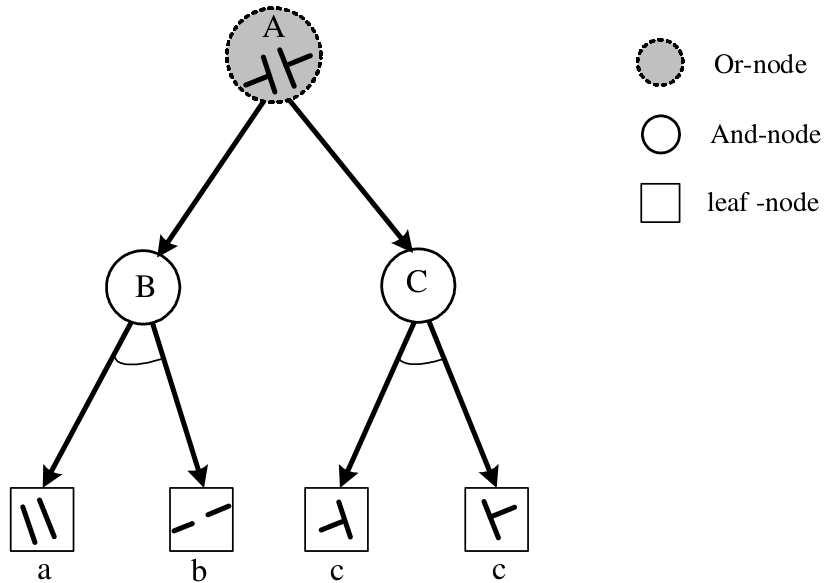
\includegraphics[width=0.4\linewidth]{./fig/fig_ii_1_3.png}
  \caption{An example of binding elements a,b,c into a larger structures A in
    two alternative ways, represented by an And-Or tree.}%
  \label{fig:ii.1.3}
\end{figure}
%

Another example, as shown in \Fig{ii.1.4}, the 6 leaf nodes can compose a set
of configurations for node $A$, which is called the ``language'' of $A$~-
denoted by $\mathbf{L}(A)$.

\begin{book_quote}{\textit{Original Texts}}
The power of composition is crucial for representing visual concepts which have
varying structures. For example, if $A$ is an object category, such as car or
chair, then $\mathbf{L}(A)$ is a set of valid designs of cars or chairs.
\end{book_quote}
%
\begin{figure}[!htpb]
  \centering
  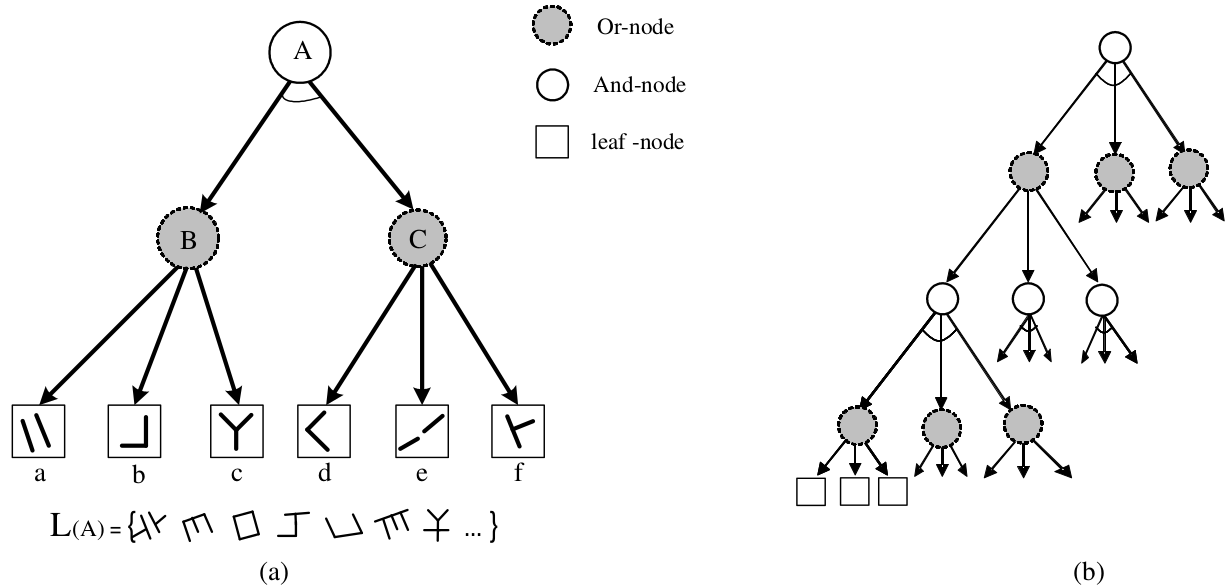
\includegraphics[width=0.8\linewidth]{./fig/fig_ii_1_4.png}
  \caption{(a) An And-node $A$ is composed of two Or-nodes $B$ and $C$, each of
    which includes three alternative leaf nodes. The 6 leaf nodes can compose a
    set of configurations for node $A$, which is called the ``language'' of
    $A$. (b) An And-Or tree (5-level branch number = 3) with 10 And-nodes, 30
    Or-nodes, and 81 leaf nodes, can produce $3^{12} = 531441$ possible
    configurations, though some may be repeated.}%
  \label{fig:ii.1.4}
\end{figure}
%

\section{Overlapping Reusable Parts}%
\label{sec:ii.1.3}
If there exists a string $\omega \in \mathbf{L}(\mathcal{G})$ that has more
than one parse tree, then $\mathcal{G}$ is said to be an \textbf{ambiguous
grammar}.
%
\begin{figure}[!htpb]
  \centering
  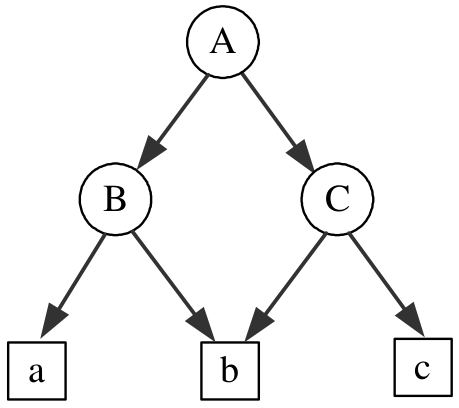
\includegraphics[width=0.35\linewidth]{./fig/fig_ii_1_5.png}
  \caption{Parts sharing and the diamond structure in And-Or graphs.}%
  \label{fig:ii.1.5}
\end{figure}
%

For example, \Fig{ii.1.6} shows two parse trees for a classic ambiguous
sentence, which has two distinct reusable parts which overlap in the
``the man''. In context, the sentence is always spoken with only one of these
meanings, so one parse is \textbf{right} while the other one is \textbf{wrong}.
\textbf{One reusable part is accepted and the other one is rejected. If we
reject one, the remaining parts do not overlap.}
%
\begin{figure}[!htpb]
  \centering
  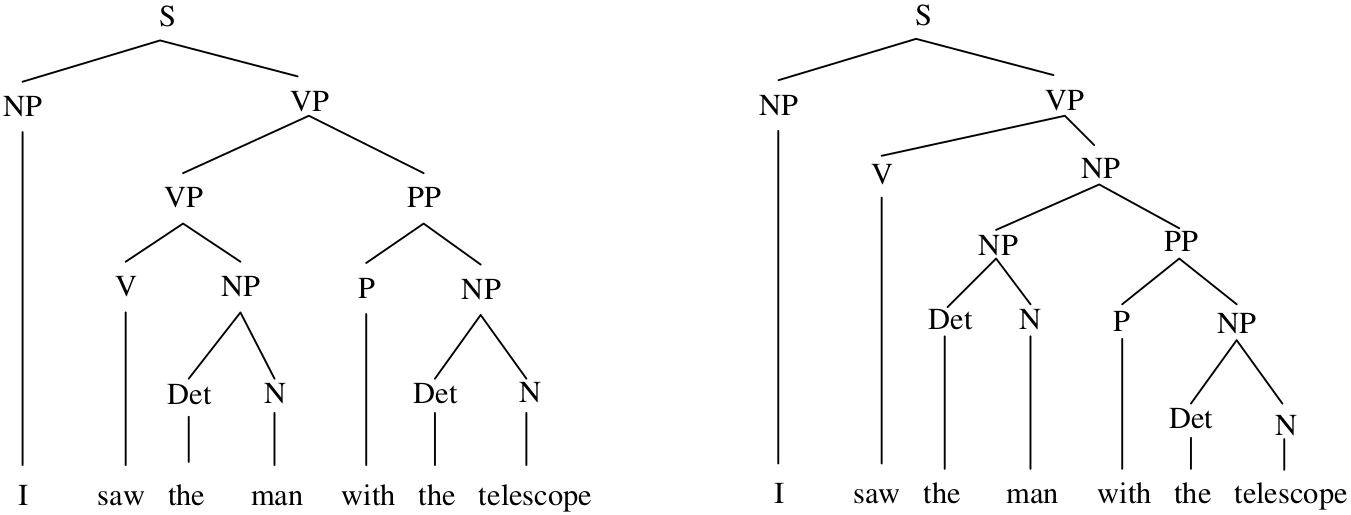
\includegraphics[width=0.8\linewidth]{./fig/fig_ii_1_6.png}
  \caption{An example of ambiguous sentence with two parse trees. The
    non-terminal nodes S, V, NP, VP denotes sentence, verbal, noun phrase, and
    verbal phrase respectively. Note that if the two parses are merged, we
    obtain a graph, not a tree, with a ``diamond'' in it as above.}%
  \label{fig:ii.1.6}
\end{figure}
%

Taking image parsing in vision, there seem to be 4 ways overlap can occur:
%
\begin{enumerate}
  \item Ambiguous scenes where distinct parses suggest themselves.
  \item High level patterns which incorporate multiple partial patterns.
  \item ``Joints'' between two high level parts where some sharing of pixels or
    edges occurs.
  \item Occlusion where a background object is completed behind a foreground
    object, so the two objects overlap.
\end{enumerate}
%
\pagebreak
%
\begin{figure}[!htpb]
  \centering
  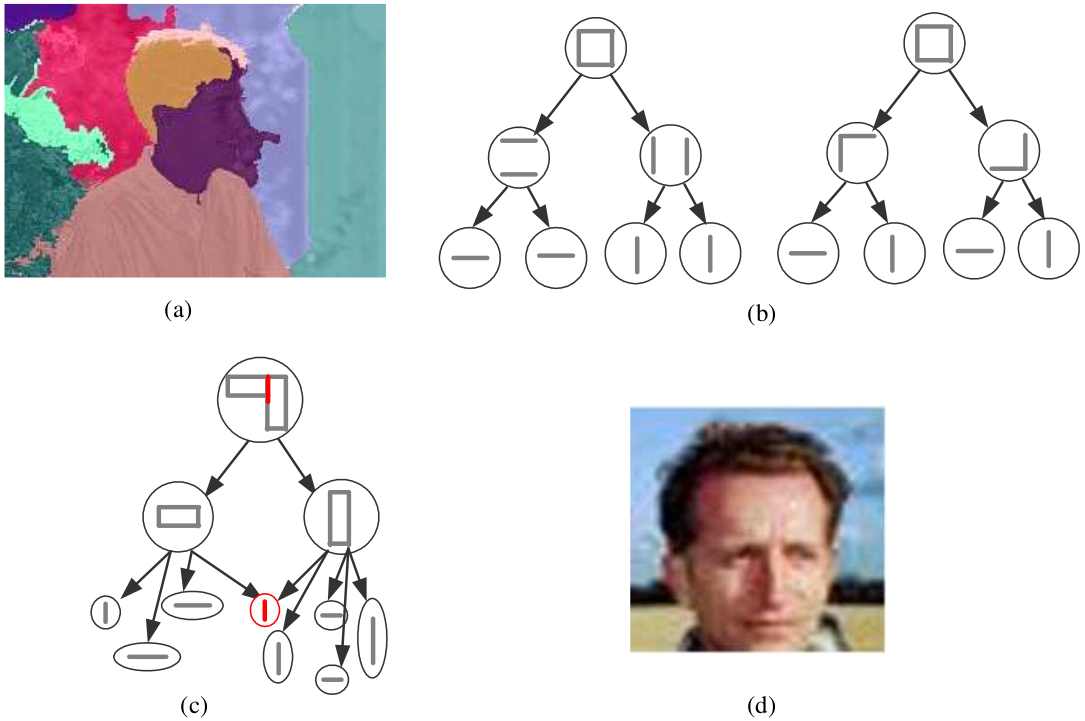
\includegraphics[width=0.8\linewidth]{./fig/fig_ii_1_7.png}
  \caption{Four types of images in which ``reusable parts'' overlap. (a) The
    Pinnocio nose is a part of the background whose gray level is close to the
    face, so it can be grouped with the face or the background. This algorithm
    chose the wrong parse. (b) The square can be parsed in two different ways
    depending on which partial patterns are singled out. Neither parse is wrong
    but the mid-level units overlap. (c) The two halves of a butt joint have a
    common small edge. A way to solve this, is to duplicate the shared edge to
    restore a tree-like parse. (d) The reconstructed complete sky, trees and
    field overlap with the face.}%
  \label{fig:ii.1.7}
\end{figure}
%
For the overlap example as shown in \Fig{ii.1.7}.d, we form duplicate images
planes carrying the two objects: this is crucial when we want to use priors to
reconstruct as much as possible of the occluded object. The right parse for
such objects should \textbf{add extra leaves} at the bottom to represent the
occluded object. The new  leaves carry \textbf{colors, textures} etc.\,
extrapolated from the visible parts of the object. Their occluded boundaries
were that \textit{gestalt school} called \textbf{amodal} contours.

\section{Stochastic Grammar}%
\label{sec:ii.1.4}
To connect with real world signals, we augment $\mathcal{G}$ with a set of
probabilities $\mathcal{P}$ as a fifth component. For example, stochastic
context free grammar (SCFG) supposes $A \in V_N$ has a number of alternative
rewriting rules,
%
\begin{align}
  \label{eq:ii.1.7}
  \tag{1.7}
  A \rightarrow \beta_1 \vert \beta_2 \vert \ldots \vert \beta_{n(A)},
  \gamma_i: A \rightarrow \beta_i
\end{align}
%
Each production rule is associated with a probability
$p(\gamma_i) = p(A \rightarrow \beta_i)$ such that:
%
\begin{align}
  \label{eq:ii.1.8}
  \tag{1.8}
  \sum^{n(A)}_{i=1} p(A \rightarrow \beta_i) = 1
\end{align}
%
This correspond to a \textbf{random branching process}. Similarly stochastic
regular grammar corresponds to a \textbf{Markov chain process}.

The probability of a parse tree:
%
\begin{align}
  \label{eq:ii.1.9}
  \tag{1.9}
  p(\mathbf{p}t(\omega)) = \prod^{n(\omega)}_{j=1} p(\gamma_j)
\end{align}
%
The probability for a string (in language) or configuration (in image)
$\omega \in \mathbf{L}(\mathcal{G})$:
%
\begin{align}
  \label{eq:ii.1.10}
  \tag{1.10}
  p(\omega) = \sum_{\mathbf{p}t(\omega)} p(\mathbf{p}t(\omega))
\end{align}
%
Therefore a $\mathcal{G} = (V_N, V_T, \mathbf{R}, S, \mathcal{P})$ produces a
probability distribution on its language
%
\begin{align}
  \label{eq:ii.1.11}
  \tag{1.11}
  \mathbf{L}(\mathcal{G}) = \{(\omega, p(\omega)):
    S \overset{\mathbf{R^*}}{\implies} \omega, \omega \in V^*_T\}
\end{align}
%
A stochastic grammar is said to be \textbf{consistent} if
$\sum_{\omega \in \mathbf{L}(\mathcal{G})} p(\omega) = 1$. This is not
necessarily true even when \Eq{ii.1.8} is satisfied for each $A \in V_N$. The
complication is caused by cases when there is a positive probability that the
parse tree may not end in a finite number of steps. For example, if we have a
production rule that expands $A$ to $AA$ or terminates to $a$,
%
\begin{align*}
  A \rightarrow AA \vert a \quad \text{with prob.}~\rho \vert (1 - \rho)
\end{align*}
%
If $\rho > \frac{1}{2}$ then $A$ expands faster than it terminates and keeps
replicating. This poses constraints for designing $\mathcal{P}$.

$\mathcal{P}$ can be learned in a supervised way from a set of
\textbf{observed parse trees} $\{\mathbf{p} t_m, m = 1, 2, \text{\ldots}, M\}$
by maximum likelihood estimation (MLE),
%
\begin{align}
  \label{eq:ii.1.12}
  \tag{1.12}
  \mathcal{P^*} = \arg \max \prod^M_{m=1} p(\mathbf{p}t)
\end{align}
%
The solution: the probability for each $A$ in \Eq{ii.1.7} is
%
\begin{align}
  \label{eq:ii.1.13}
  \tag{1.13}
  p(A \rightarrow \beta_i) = \frac{\#(A \rightarrow \beta_i)}{\sum^{n(A)}_{j=1} \#(A \rightarrow \beta_i)}
\end{align}
%
where $\#(A \rightarrow \beta_i)$ is the number of times a rule is used in all
the $M$ parse trees.

In a unsupervised learning case, when the observation is
\textbf{a set of strings} without parse trees, one can still follow the MLE
above with an expectation-maximization (ME) algorithm. It was shown
in\cite{zhiyichi1998} that the MLE of $\mathcal{P}$ can rule out infinite
expansion and produce a consistent grammar.

In \Fig{ii.1.3}, one can augment the two parses by probabilities $\rho$ and
$1 - \rho$, written as a stochastic production rule:
%
\begin{align}
  \label{eq:ii.1.14}
  \tag{1.14}
  A \rightarrow a \cdot b \vert c \cdot c; \quad \rho \vert (1 - \rho)
\end{align}
%

%================================================================= Bibliography
\bibliographystyle{plain}
\bibliography{./part_ii.bib}

\end{document}
